\documentclass[conference]{IEEEtran}
\IEEEoverridecommandlockouts
% The preceding line is only needed to identify funding in the first footnote. If that is unneeded, please comment it out.
\usepackage{cite}
\usepackage{amsmath,amssymb,amsfonts}
\usepackage{algorithmic}
\usepackage{graphicx}
\usepackage{textcomp}
\usepackage{xcolor}
\usepackage[spanish]{babel}
\usepackage{circuitikz}
\usepackage{float}
\usepackage{hyperref}

\def\BibTeX{{\rm B\kern-.05em{\sc i\kern-.025em b}\kern-.08em
    T\kern-.1667em\lower.7ex\hbox{E}\kern-.125emX}}
\begin{document}

\title{Trabajo Práctico "Disipadores"\\
{\footnotesize \textsuperscript{}Curso 2023 - Tecnología de los Materiales Electrónicos}
\thanks{}
}

\author{\IEEEauthorblockN{1\textsuperscript{st} Ramiro Belsito}
\IEEEauthorblockA{\textit{Estudiante} \\
\textit{Instituto Tecnológico de Buenos Aires}\\
Buenos Aires, Argentina\\
rabelsito@itba.edu.ar}
\and
\IEEEauthorblockN{2\textsuperscript{nd} Facundo Caviglia}
\IEEEauthorblockA{\textit{Estudiante} \\
\textit{Instituto Tecnológico de Buenos Aires}\\
Buenos Aires, Argentina \\
fcaviglia@itba.edu.ar}}

\maketitle


\begin{abstract}
En el siguiente informe se analizará la utilidad de dos disipadores proveídos por la cátedra
para el buen funcionamiento de un regulador de tensión con encapsulado TO220.
\end{abstract}

\section{Introduction}
Se analizará la resistencia térmica de estos por medio de la práctica y se comparará con los valores 
obtenidos por medio de las ecuaciones teóricas y la hoja de datos del fabricante. Para esto realizamos un
circuito detallado a continuación, de modo que se caliente y forzar la activación del el circuito interno de
protección por temperatura. Sobre el mismo conectamos en serie un amperímetro para encontrar la corriente
que circula por el LM317 con estrangulamiento térmico,la cual esta en relación directa con la potencia (Q).
Con estos datos se realizará el circuito térmico equivalente y se estudiará la influencia del posicionamiento
del disipador, frente a la posición óptima.
\begin{figure}[h]
    \centering
    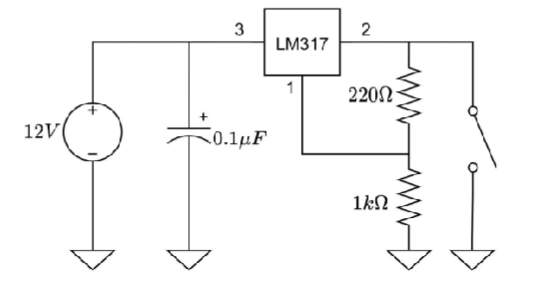
\includegraphics[width=0.25\textwidth]{CircuitoDeMedicion.png}
    \caption{Circuito de Medición}
\end{figure}

\section{Forma y Dimensiones}
\begin{figure}[H]
    \centering
    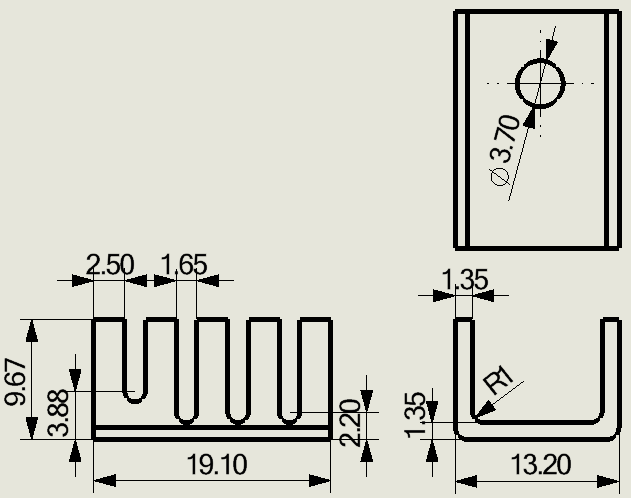
\includegraphics[width=0.25\textwidth]{disipadorFacu.png}
    \caption{Plano del disipador 1 ($*^1$)}
\end{figure}
\begin{figure}[H]
    \centering
    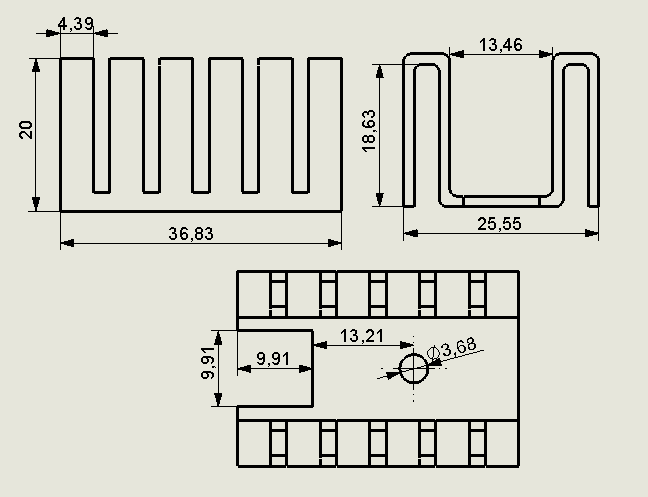
\includegraphics[width=0.25\textwidth]{PlanoRamiCompleto.png}
    \caption{Plano del disipador 2 ($*^2$)}
\end{figure}
Ambos disipadores son estampados sobre una plancha de aluminio anodizado, y luego tratado con otros 
procesos mecánicos para obtener la forma de cada uno. Por su método de fabricación cada disipador
es una pieza única, a diferencia de los fabricados por extrusión, que son piezas continuas cortadas 
a la medida requerida

\section{Cálculos Teóricos}
La resistencia térmica de un disipador dada por convección natural se calcula mediante la siguiente
ecuación:
\begin{equation}
    R_{sa} = \frac{1}{1,34\cdot A_s}\cdot (\frac{d_v}{\Delta T})^{\frac{1}{4}}
\end{equation}
Donde $A_s$ es la superficie de contacto entre el disipador y el aire, $d_v$ es la distancia vertical.

\subsection{Disipador 1 ($*^1$)}
La temperatura de trabajo máxima del LM317 se encuentra en 150°C, y la temperatura ambiente
se presume a 25°C. Obteniendo asi $\Delta T = 125$°C.
Meidante la función de análisis de propiedades físicas del modelado en SolidWorks, se obtuvieron
los datos pertinentes al cálculo de la resistencia:
$A_d$ = 1196,35 $mm^2$
$d_v$ = 9,67 $mm$.

\begin{align*}
    R_{sa} = 58,5 C/W
\end{align*}

\subsection{Disipador 2 ($*^2$)}
Utilizando la misma metodología que en el Disipador 1 ($*^1$) y frente a las mismas condiciones,
se obtuvieron los siguientes datos:
$A_d$ = 6915,40 $mm^2$
$d_v$ = 36,83 $mm$.
\begin{align*}
    R_{sa} = 14,1 C/W
\end{align*}
\subsection{Circuito Térmico Equivalente}

\begin{figure}[H]
    \centering
    \begin{circuitikz}[american, cute inductors, scale=0.45]
        \draw (0,0) to[I, l=$Q$] (0,3)
                    to[R, l=$R_{jc}$] (4,3)
                    to[R, l=$R_{cs}$] (8,3)
                    to[R, l=$R_{sa}$] (8,0)
                    to[short] (0,0);
    \end{circuitikz}
    \caption{Circuit diagram}
\end{figure}


\section{Mediciones Experimentales}
A continuación pueden observarse las mediciones llevadas a cabo en el laboratorio. Primero,
Se estudiará la corriente en la salida del LM317 y su tensión, así teniendo idea de la potencia
que está disipando el componente. Además, se analizará el comportamiento del disipador con la presencia 
de grasa siliconada. Luego, se cambiaron los disipadores a distintas posiciones, y 
se concluirá su posición más eficiente para la convección natural.


\begin{table}[htbp]
    \caption{Mediciones sobre los Disipadores}
    \begin{center}
    \begin{tabular}{|c|c|c|c|}
    \hline
    \textbf{Mediciones} & \multicolumn{3}{|c|}{\textbf{Número de Disipador}} \\
    \cline{2-4} 
    \textbf{de Laboratorio} & \textbf{\textit{Sin Disipador}} & \textbf{\textit{Disipador 1 ($*^1$)}} & \textbf{\textit{Disipador 2 ($*^2$)}} \\
    \hline
    $I_{m\acute{i}n}$ (sin grasa) & 0,21A & 0,45A & 0,9A \\
    \hline
    $I_{m\acute{i}x}$ (con grasa) & - & 0,52A & 1,11A \\
    \hline
    $V$ & 12v & 12v & 11,96v \\
    \hline
    $Q$ (sin grasa) & 2,52W & 5,4W & 10,76W \\
    \hline
    $Q$ (con grasa) & - & 6,24W & 13,28W \\
    \hline
    \end{tabular}
    \label{tab1}
    \end{center}
    \end{table}

    Se puede observar mediante la tabla que la aplicación de grasa siliconada mejora la transferencia de calor entre el 
    componente y el disipador. Esto se debe a que la grasa ayuda a llenar los espacios microscópicos y las irregularidades 
    superficiales, mejorando el contacto térmico y, por ende, aumentando la eficiencia de la disipación de calor. En el caso
    del Disipador 1 ($*^1$), la mejora es de un 23\%, mientras que en el Disipador 2 ($*^2$) es de un 15\%.\\ \\
    A continuación puede verse una comparación entre las posiciones de los disipadores (sin grasa siliconada), y su 
    influencia en la disipación de calor. La posición 1 se refiere al disipador en vertical, la posición 2 en 
    horizontal, y la posición 3 en diagonal.

    \begin{table}[htbp]
        \caption{Diferencias entre las posiciones del Disipador}
        \begin{center}
        \begin{tabular}{|c|c|c|}
        \hline
        \textbf{Mediciones} & \multicolumn{2}{c|}{\textbf{Número de Disipador}} \\
        \cline{2-3}
        \textbf{de Laboratorio} & \textbf{\textit{Disipador 1 ($*^1$)}} & \textbf{\textit{Disipador 2 ($*^2$)}} \\
        \hline
        $I_{m\acute{i}n}$ (posicion 1) & 0,45A & 0,9A \\
        \hline
        $I_{m\acute{i}n}$ (posicion 2) & 0,43A & 0,82A \\
        \hline
        $I_{m\acute{i}n}$ (posicion 3) & 0,44A & 0,85A \\
        \hline
        
        \end{tabular}
        \label{tab1}
        \end{center}
    \end{table}

    La eficiencia de la disipación de calor puede variar dependiendo de la orientación del disipador. 
    En este experimento, puede observarse que para ambos disipadores, la posición vertical es la más eficiente,
    seguida por la posición diagonal y por último la posición horizontal. Esto se debe a que la posición vertical
    permite que el aire caliente ascienda, y el aire frío descienda, generando una corriente de convección natural
    que ayuda a disipar el calor. En cambio, en la posición horizontal, el aire caliente queda atrapado en el disipador,
    y el aire frío no puede ingresar, por lo que la disipación de calor es menos eficiente.\\ \\

    A continuación se puede observar una comparación entre las resistencias térmicas teóricas y las experimentales.
    \begin{table}[htbp]
        \caption{Comparación entre las Resistencias Térmicas}
        \begin{center}
        \begin{tabular}{|c|c|c|}
        \hline
        \textbf{Resistencias} & \multicolumn{2}{c|}{\textbf{Número de Disipador}} \\
        \cline{2-3}
        \textbf{térmicas} & \textbf{\textit{Disipador 1 ($*^1$)}} & \textbf{\textit{Disipador 2 ($*^2$)}} \\
        \hline
        $R_{sa}$ (hoja de datos) & 28 C/W & 12,4 C/W \\
        \hline
        $R_{sa}$ (teórica) & 58,5 C/W & 14,1 C/W \\
        \hline
        $R_{sa}$ (experimental) & 23,1 C/W & 11,6 C/W \\
        \hline
        \end{tabular}
        \label{tab1}
        \end{center}
    \end{table}

    \section{Conclusiones}

    Mediante los experimentos que llevamos a cabo y sus resultados, podemos concluir que la utilización de grasa 
    siliconada mejora la transferencia de calor entre el componente y el disipador en un promedio de 20\%. Además,
    probando distintas posiciones del disipador, concluimos que la posición vertical es la más eficiente,
    \\La posición vertical del disipador (posición 1) mostró ser la más efectiva para disipar calor. En esta orientación, 
    la convección natural permite un flujo más eficiente del aire caliente hacia arriba, alejándolo del componente que 
    genera calor y facilitando su disipación hacia el entorno. Por último, cabe aclarar que la utilización de un
    disipador es fundamental para la disipación de calor de un componente, ya que sin él, el componente podría elevar
    su temperatura por encima de la temperatura máxima de trabajo, y dañarse. \\Una observación importante del experimento
    es que la ventilación forzada aumenta activamente el flujo de aire alrededor del componente caliente, mejorando 
    significativamente la disipación de calor al eliminarlo más rápido. Simulamos una confinación del circuito posicionandolo
    en una caja cerrada, y la corriente mínima a la salida fue menor a la obtenida sin confinación. Luego, ventilamos
    manualmente el circuito, y la corriente mínima a la salida fue mayor a la obtenida sin ventilación.
    \\También, puede verse en los resultados
    experimentales que cualquiera sea la posición del disipador, la potencia disipada siempre es mayor a la de un
    componente sin disipador, por lo que la utilización de un disipador siempre es recomendable.

    \section{Apéndice}
    ($*^1$) Disipador 1: Modelo 551002B00000G de la marca Boyd \\
    ($*^2$) Disipador 2: Modelo 274-1AB de la marca Wakefield-Vette \\
    \section{Bibliografía}
    \begin{itemize}
        \item \href{https://www.digikey.com/en/products/detail/wakefield-vette/274-1AB/340321}{Hoja de Datos Disipador 1}
        \item \href{https://es.farnell.com/boyd/551002b00000g/heat-sink/dp/1339511}{Hoja de Datos Disipador 2}
    \end{itemize}

\end{document}
